\section{Elementi di architettura Linux e Shell Scripting}
\subsection{Command-line Interface}
\subsubsection{Introduzione}
L'interfaccia a linea di comando (\textbf{command-line interface} o \textbf{CLI}) si occupa di processare comandi forniti in forma testuale (text-based). 
Il programma che gestisce l'interfaccia e' noto come \textbf{command-line interpreter} o command-line processor. 
I sistemi operativi implementano una cli all'interno di una \textbf{shell} per consentire all'utente
di interagire con le funzioni e i servizi messi a disposizione dal sistema operativo,
offrendo di fatto un'interfaccia interattiva verso quest'ultimo. Ogni shell e' dotata di un proprio linguaggio
con relativa sintassi, di fatto general purpose, con tutte le caratteristiche dei piu'
comuni linguaggi in grado di risolvere una qualunque tipologia di problema. Questo pero' risulta particolarmente
efficace nel processo di automatizzazione di procedure, job , set di operazioni per l'amministrazione di 
sistema e non solo. La shell indica la predisposizione a ricevere comandi attraverso una stringa di caratteri
visualizzati nella parte iniziale della prima linea vuota. Questa stringa e' detta \textbf{prompt}.
Questa tipicamente processa \textbf{comandi} e \textbf{argomenti}

\subsubsection{Comandi}
	\subparagraph{Keyword}
	E' un comando che ha il compito di modificare l'esecuzione di altri comandi
	(es. misurare il tempo di esecuzione, innescare un ciclo)
	\subparagraph{Built-in}
	Questa categoria comprende comandi direttamente eseguiti dal codice interno di una shell che li
	interpreta convertendoli in azioni sul sistema operativo. Un esempio tipico e' costituito dai comandi
	per la navigazione del filesystem.
	\subparagraph{Esterni}
	Un comando esterno e' un file eseguibile che viene localizzato e messo in esecuzione dalla shell
	(tipicamente come processo figlio). La shell puo' poi attenderne o meno la conclusione prima di 
	accettare nuovi comandi.
	\subparagraph{Alias}
	La shell consente di fare aliasing di comandi o set di comandi, di fatto convertendo l'alias nella
	stringa precedentemente associata.
	\subparagraph{Funzioni}
	Una funzione e' un'intera sequenza di comandi shell, alla quale viene attribuito un nome ed eventuali
	parametri in input.


{\pagebreak}

\subsubsection{Documentazione dei comandi}
Per conoscere il funzionamento di una determinata applicazione o di un comando esterno e' possibile fare 
rifermento a 'pagine di manuale' (man pages) relative al suo utilizzo e configurazione. 
Il comando che permette di fare cio' e' \texttt{man}. L'installazione di un pacchetto software (applicazione)
comprende le relative pagine di manuale, ad eccezione pero' dei comandi built-in in quanto gia' implementati 
nel codice della shell, e non installati indipendentemente questi, contrariamente al resto delle 
applicazioni, non possiedono delle man pages accessibili tramite man, ma un sommario del loro funzionamento puo'
essere visualizzato con il comando \texttt{help <built-in>}.

\subparagraph{Categorie di man pages}
Una installazione standard di UNIX mette a disposizione svariate \textbf{pagine di manuale} raggruppate in
sezioni:
	\begin{enumerate}
		\item User commands (Executables programs or shell commands)
		\item Chiamate al sistema operativo (System calls)
		\item Funzioni di libreria (Library calls)
		\item File speciali (Special files, \texttt{/dev/*})
		\item Formati dei file. dei protocolli e delle relative strutture C
		\item Giochi
		\item Varie: macri, header, filesystem, concetti generali
		\item Comandi per utenti privilegiati per amministrazione di sistema
		\item Kernel Routine
	\end{enumerate}

\subparagraph{Sintassi per l'accesso alle man pages}
In generale l'accesso alla man pages si ottiene con il comando \\
\begin{center}
	\texttt{man <nome della pagina>}
\end{center}
dove spesso il nome della pagina coincide con il comando o il nome del file di configurazione che essa documenta.
Altre opzioni utili:
\begin{center}
\begin{tabular}{ll}
	\texttt{man -a <comando>} & cerca in tutte le sezioni \\
	\texttt{man <sez.> <comando>} & cerca nella sezione specificata \\
	\texttt{man -k <keyword>} & cerca tutte le pagine attinenti alla parola chiave specificata \\
\end{tabular}
	
\end{center}

\subsubsection{Argomenti}
Ogni comando, sia built-in che esterno, puo' accedere ai caratteri che seguono la propria invocazione sulla
command line, per fare cio' la shell inserisce in memoria l'ARGV prima di generare il processo. Questi sono
generalmente nella forma di gruppi di caratteri separati da spazi. Tra questi ne riconosciamo un particolare
tipo, caratterizzato generalmente dal carattere prefisso \texttt{'-'} noto come \textbf{opzione}. Questo 
generalmente non ' un vero e proprio dato da elaborare, ma piu' un modo di specificare una variante al 
comportamento del comando che si sta chiamando. Piu' opzioni possono essere solitamente raggruppate in un'unica
stringa.

\subsubsection{History e attivita'}
\texttt{history} mostra la 'storia' di tutti i comandi eseguiti in un terminale. 
E' possibile richiamare un comando utilizzando la freccia-su, facendo comparire quelli piu' recentemente utilizzati. Un altro approccio sfrutta
la ricerca interattiva utilizzando un prompt \textbf{reverse-i-search} , attivabile con \texttt{CTRL-r}. 
Una volta inviduato, lo si puo' lanciare direttamente (invio) o editare (freccie dx/sx). \\
Un'altro comando interessante e' invece \texttt{script} il quale permette invece di catturare su un file 
una sessione di lavoro, esattamente come compare a video, risultati compresi.\\
Per terminare una sessione con il terminale e' sufficiente digitare \texttt{exit} o premete \texttt{CRTL-d}.

\subsubsection{Comandi di base relativi al filesystem} 
\begin{center}
	\begin{tabular}{c|c}
		\hline
		\texttt{ls} & elenca i file (list files)\\ 
		\texttt{cd} & cambia directory (change directory)\\ 
		\texttt{pwd} & mosta la directory corrente (print working directory)\\ 
		\texttt{df} & mostra lo spazio utilizzato e disponibile su ogni filesystem\\ 
		\texttt{du} & visualizza l'uso di spazio di un file o di una directory\\ 
		\texttt{rm} & rimuove un link ad un file \\ 
		\texttt{cp} & copia un file o piu' file in una directory \\ 
		\texttt{mv} & sposta un file o piu' file in una directory \\ 
		\texttt{ln} & crea un link ad un file \\ 
		\texttt{mkdir} & crea una directory \\ 
		\texttt{rm} & cancella una directory \\ 
		\hline
	\end{tabular}
\end{center}
\noindent
\subparagraph{Navigazione nel filesystem}
E' importante ricordare che ogni directory di UNIX contiene due directory speciali:
\begin{center}
	\begin{tabular}{cl}
		\texttt{.} & punta la directory stessa \\ 
		\texttt{..} & punta alla directory genitore (parent) \\ 
	\end{tabular}
\end{center}
Ogni percorso che inizia con la barra viene considerato \textbf{assoluto}, cioe' relativo
alla radice, mentre se inizia con qualsiasi altro carattere viene considerato relativo
alla directory corrente.\\

\subparagraph{\textbf{Tip}}
	Il comando \texttt{cd -} permette di tornare alla directory precedente l'ultima chiamata di \texttt{cd}.

\subsubsection{Shell expansion}
La shell opera secondo un procedimento di \emph{espansione}. Individua sequenze speciali
contrassegnate da \emph{meta-caratteri}, i quali non vengono presi a valore nominale.
Interpreta il significato della sequenza speciale, sostituendo il risultato 
dell'interpretazione al posto della sequenza. Viene cosi creata una riga di comando
differente da quella digitata. Se un'espansione fallisce la sequenza e' solitamente
lasciata inalterata sulla riga di comando.\\

Ci sono ben \textbf{12 passi} che svolgono tipologie di manipolazioni diverse della riga
di comando, in una sequenza precisa. Alcuni/tutti questi passi possono essere
saltati per mezzo del \textbf{quoting}, cioe' proteggendo i meta-caratteri da non
interpretare, per mezzo di altri caratteri speciali quali:
\textbf{apici} \texttt{'} ,
\textbf{doppi apici} \texttt{"},
\textbf{backslash} \texttt{\textbackslash}.


\subparagraph{1 - Tokenizzazione}
La riga di comando viene suddivisa in \textbf{token} usando come separatori un elenco
fisso di metacaratteri:
\begin{center}
	\texttt{SPACE TAB NEWLINE ; ( ) < > | \& } 
\end{center}
Questi possono essere:
\begin{itemize}
	\item Stringhe
	\item Parole chiave
	\item Caratteri di redirezione
	\item Carattere "\textbf{:}"
\end{itemize}
Notare che se una parte viene racchiusa fra apici singoli, i passi dal 2 al 10 
veranno ignorati.

\subparagraph{2 - Primo token alias}
La shell cerca il primo token nella lista degli alias. Se lo trova, questo viene
espanso e il procedimento ricomincia dal passo 1. Notare che la shell impedisce di 
espandere lo stesso alias per piu' di una volta, cosi da evitare chiamate ricorsive
infinite. E' importante notare che l'espansione non avviene sulle porzioni di command
line racchiuse da doppi apici.


\subparagraph{3 - Primo token keyword}
Se il primo token e' un parola chiave che da' inizio a un comando composto es.
\begin{center}
	\texttt{IF WHILE FUNCTION $\{$ $($}
\end{center}
la shell predispone l'ambiente per il comando composto e ne va a leggere il primo token.
Come per il passo 2, questo non viene eseguito per porzioni racchiuse da doppi apici.

\subparagraph{4 - Brace expansion}
L'espansione delle parentesi viene utilizzata per generare stringhe arbitrarie.
Permette infatti di creare argomenti multipli, a partire da un singolo argomento di 
command line. Le stringhe specificate vengono utilizzate per creare tutte le possibili 
combinazioni, alle quali e' possibile associare un preambolo e un postscript.
Il preambolo viene prefisso a ogni stringa contenuta fra le parentesi, successivamente,
a queste viene aggiungo il postscript come suffisso, espandendo da sinistra a destra.

\begin{lstlisting}[language=bash,basicstyle=\ttfamily,frame=single]
$ echo last{mce,boot,xorg}.log
lastmce.log lastboot.log lastxorg.log

where last is Preamble and .log is the postscript
\end{lstlisting}


\subparagraph{5 - Tilde expansion}
Se c'e' un token nella forma \texttt{~username}, viene sostituito con la \texttt{HOME} 
directory dell'utente \texttt{username} (se username e' vuoto, si utilizza l'utente
corrente)

\subparagraph{6 - Parameter expansion}
Il carattere \texttt{\$} puo' marcare l'inizio di diverse espansioni:
\begin{itemize}
	\item paramter expansion
	\item command substitution
	\item arithmetic expansion
\end{itemize}
L'esempio piu' semplice di PE e' la sostituzione della stringa \texttt{\$NAME} con il 
valore contenuto nella variabile \texttt{NAME}.
Questi quattro passaggi (6..9) sono eseguiti anche sulle parti 
di riga racchiuse tra doppi apici.

\subparagraph{7 - Command substitution}
Il token \texttt{\$(comando)} ha il seguente effetto:
\begin{itemize}
	\item viene creata una subshell 
	\item si esegue il comando nella subshell appena creata 
	\item lo \texttt{stdout} di \texttt{comando} viene posto sulla riga di comando
		al posto del token originale, a parte eventuale righe vuote alla fine
\end{itemize}
Questi quattro passaggi (6..9) sono eseguiti anche sulle parti 
di riga racchiuse tra doppi apici.

\subparagraph{8 - Arithmetic expansion}
Il token \texttt{((expr))} viene sostituito col risultato della valutazione di 
\texttt{expr}, un'espressione aritmetica. \texttt{expr} viene trattata come se fosse
racchiusa tra doppi apici (quindi subisce solo i passi 6 e 7).\\ 
Questi quattro passaggi (6..9) sono eseguiti anche sulle parti 
di riga racchiuse tra doppi apici.

\subparagraph{9 - Process substitution}
Il token \texttt{<(comando)} o \texttt{>(comando)} ha questo effetto:

\begin{itemize}
	\item viene eseguito \texttt{comando} in modo concorrente e asincrono rispetto al comando
		all'inizio della riga.
	\item il suo input o output appare come un nome di file tra gli argomenti di tale comando.
\end{itemize}
Questi quattro passaggi (6..9) sono eseguiti anche sulle parti 
di riga racchiuse tra doppi apici.

\begin{wrapfigure}{L}{4in}
	\begin{center}
		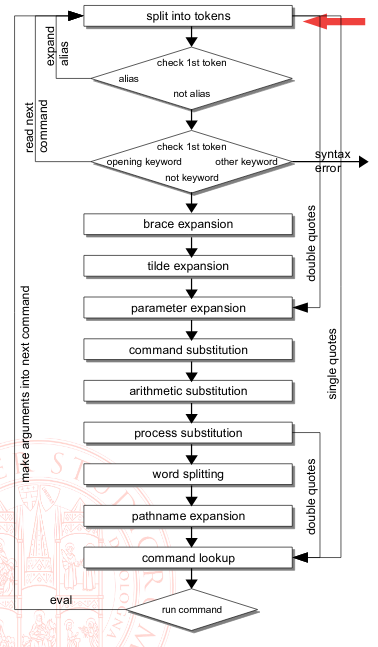
\includegraphics[width=0.6\textwidth]{img/shell-expansion.png}
		\caption{Shell expansion}
	\end{center}
\end{wrapfigure}
\subparagraph{10 - Word splitting}
I risultati dei passi 6..9 sono esaminati, e separati in \emph{word} indipendenti. I caratteri riconosciuti
come separatori sono contenuti nella variabile di ambiente \textbf{IFS} (\emph{Internal Field Separator})
Questa di default e' impostata per riconoscere come caratteri di separazione :
\begin{center}
	\texttt{<space> <tab> <newline>}
\end{center}
Questo passo non viene eseguito sulle parti di riga racchiuse fra doppi apici.


\subparagraph{11 - Pathname expansion}
Ogni word viene esaminata e se contiene uno dei caratteri

\begin{itemize}
	\item \texttt{*}
	\item \texttt{?}
	\item \texttt{$[$}
\end{itemize}
viene considerata un \textbf{pattern} e sostituita con tutti i nomi di file che vi corrispondono.
Questo passo non viene eseguito sulle parti di riga racchiuse fra doppi apici.


\subparagraph{12 - Quote removal ed esecuzione}
Vengono rimosse tutte le occorrenze di caratteri di quoting "usate" effettivamente, quindi non protette
da altri quoting o generate dai passi 6..9. Vengono poi impostati gli stream in caso di redirezione e viene
poi cercato il comando in quest'ordine:
\begin{itemize}
	\item funzioni
	\item built-it
	\item eseguibili in \texttt{\$PATH}
\end{itemize}

\subsubsection{Tipologie di comandi e ricerca}
Per distinguere quale tipo di comando viene eseguito da una shell e' possibile utilizzare il comando 
\texttt{type}.

\begin{lstlisting}[language=bash,basicstyle=\ttfamily,frame=single]
$ type -a echo
echo is a shell builtin
echo is a /bin/echo
\end{lstlisting}
E' possibile alterare l'ordine di default con i seguenti meccanismi:
\begin{itemize}
	\item backslash \texttt{\textbackslash} davanti al comando: previene solo l'espansione degli alias.
	\item keyword \texttt{builtin}: previene l'espansione degli alias e l'uso di funzioni e invoca
		l'esecuzione del builtin specificato, se esite.
	\item comando \texttt{unalias}: cancella un alias definito in precedenza
\end{itemize}
Per quanto riguarda invece i comandi esterni, la shell utilizza tra le variabili di ambiente comuni,
la variable \texttt{\$PATH} per eseguire la ricerca dei comandi nel filesystem. La sua struttura e' quella
di un elenco di directory separate da carattere "\textbf{:}".
\begin{center}
	\texttt{PATH:/bin:/usr/bin:/sbin}
\end{center}
Nel caso di eseguibili omonimi in directory diverse, il sistema utilizza (appoggiandosi ad una lista ordinata)
la prima istanza che trova. Il comando \texttt{which} in questo caso ci permette di distinguere quale versione
si sta utilizzando.


\begin{lstlisting}[language=bash,basicstyle=\ttfamily,frame=single]
$ which passwd
/usr/bin/passwd
\end{lstlisting}
Per consentire automaticamente l'esecuzione di programmi presenti in una determinata directory, il percorso
di questa deve essere presente nella variable d'ambiente \texttt{\$PATH}.
\textbf{Tip:} non e' buona norma inserire intere directory nella variable \texttt{\$PATH}, e' 
sempre meglio utilizzare
percorsi espliciti cosi' da non incorrere in errori inaspettati.
